\section{Translations}
To have a scalable application it is necessary to easily be able to translate the text to different languages.
For this purpose we have used i18next, which is an internationalization framework for JavaScript.
It is supported for many different frameworks like React, React Native, .net, Angular and many more \cite{react-i18next}.
Instead of hardcoding the text on every page, we wrap the export of the component in the function withTranslations which injects the function t into the props of the component.  

\begin{lstlisting}[caption={Translated header when registering as a user.}, captionpos=b, label={withTranslationsUserForm}]
    import { withTranslation } from "react-i18next";

    function UserForm(props){
        const { t, classes } = props;

        return (
            <Container maxWidth="sm">
               <div className={classes.paper}>
                  <Typography align="center" variant="h4">
                      {t('registerasauser')}
                  </Typography>
               ...
        );
    }

    export default withTranslation()(withStyles(styles)(UserForm))
\end{lstlisting}
\noindent
In \autoref{withTranslationsUserForm} is the translation for the header on the register page.
The \texttt{withTranslation()} component will then look in the translation files to find the correct translation for "registerasauser". 
A screenshot of the files can be seen on \autoref{fig:translationfiles}.
\begin{figure}
    \centering
    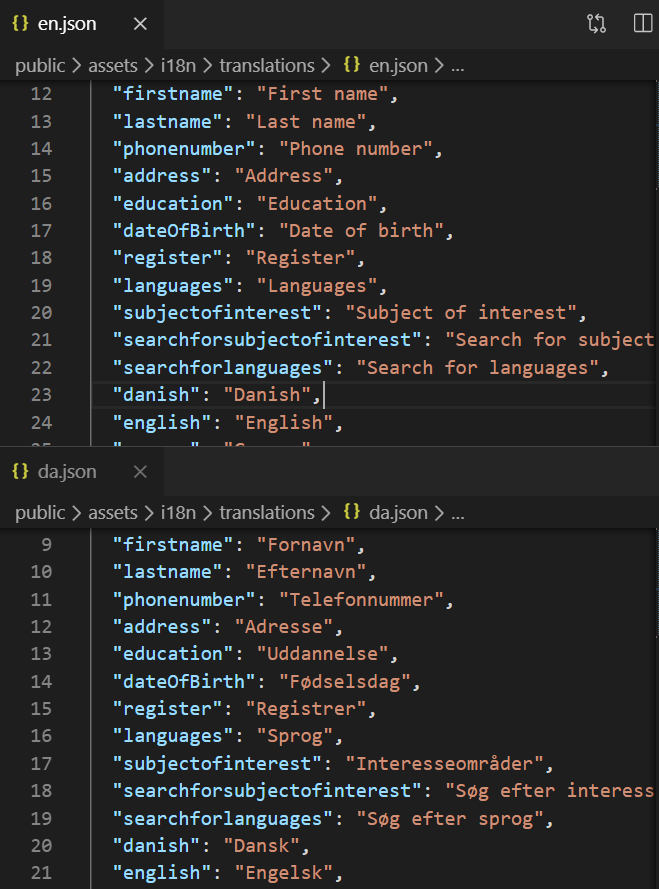
\includegraphics[scale=0.5]{figures/translations.PNG}
    \caption{The Danish and English translation files}
    \label{fig:translationfiles}
\end{figure}
\noindent
To add an additional language all that needs to be done is to make a new file and translate all the lines. 
It is not necessary to refactor any code to add additional languages.
